\documentclass{IEEEtran}
\usepackage{filecontents}
\usepackage{lipsum}
\usepackage[utf8]{inputenc}
\usepackage{graphicx} % for image
\usepackage{color} % for image (?)
\usepackage{amsmath}
\DeclareGraphicsExtensions{.png}

% correct bad hyphenation here
\hyphenation{op-tical net-works semi-conduc-tor}


\begin{document}
%
% paper title
% can use linebreaks \\ within to get better formatting as desired
\title{RNA (Título Provisório)}
%
%
% author names and IEEE memberships
% note positions of commas and nonbreaking spaces ( ~ ) LaTeX will not break
% a structure at a ~ so this keeps an author's name from being broken across
% two lines.
% use \thanks{} to gain access to the first footnote area
% a separate \thanks must be used for each paragraph as LaTeX2e's \thanks
% was not built to handle multiple paragraphs
%

\author{Fábio~Juste, Geraldo~Gusmão e Luiz~Le~Roy - ~\IEEEmembership{PUC Minas}
        % <-this % stops a space
\thanks{Texto finalizado em 15 de fevereiro de 2014.}}

% The paper headers
\markboth{Journal of \LaTeX\,~Vol.~X, No.~Y, Fevereiro~2014}%
{Shell \MakeLowercase{\textit{et al.}}: Bare Demo of IEEEtran.cls for Journals}

% make the title area
\maketitle

\begin{abstract}
%\boldmath
O artigo ...
\end{abstract}

\begin{IEEEkeywords}
Sistemas ...
\end{IEEEkeywords}

\IEEEpeerreviewmaketitle

\section{Introdução}
\IEEEPARstart{O} objetivo deste trabalho é construir uma rede neural baseada nos conceitos de conjuntos nebulosos ou Fuzzy,  utilizando neurônios lógicos AND e OR, propostos por Pedricz e Hirota.
Para a construção tomamos como base uma  tabela de valores com quatro valores para as entradas e uma saída para cada combinação destes valores. Utilizamos um algoritmo PSO – Particle Swarm Optmization para treinamento da rede.  A escolha do algoritmo de treinamento mostrou resultados satisfatórios quanto a performance computacional  e convergência em até 150 iterações.

\section{Neurônios Lógicos}
Utilizamos uma topologia composta por blocos de neurônios formados por três neurônios (figura \ref{neur}) , sendo dois neurônios na entrada associados a um neurônio de saída. Os neurônios de entrada satisfazem a funções lógicas AND e OR e o neurônio de saída satisfaz a função lógica OR. A função AND é modelada  através do uso dos conceitos de funções de agregação disjuntiva (t-norma) e a função OR  a partir dos conceitos de funções de agregação conjuntiva (s-norma).

Para obter as funções conjuntivas utilizamos a equação \ref{conj}.
\begin{equation} \label{conj}
  f(x) \leq min(x) = min(x_1,x_2, ..., x_n)
\end{equation}

Para obter as funções disjuntivas utilizamos a equação \ref{disj}.
\begin{equation} \label{disj}
  f(x) \geq max(x) = max(x_1,x_2, ..., x_n)
\end{equation}

\begin{figure}[ht!]
	\centering
	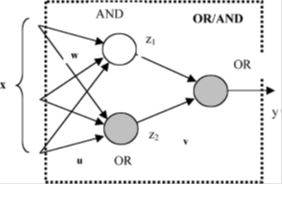
\includegraphics{or-and.png}
	\caption{Neurônios OR / AND}
	\label{neur}
\end{figure}

\section{Arquitetura da rede}
A escolha da arquitetura considerou como requisito a capacidade da rede comportar-se como um neurônio AND ou então como OR, em função do resultado de saída desejado. 

Analisamos duas arquiteturas propostas:

Arquitetura 1: com convergência,  mas com erros em um grande número de testes (figura \ref{arq1}).
\begin{figure}[ht!]
	\centering
	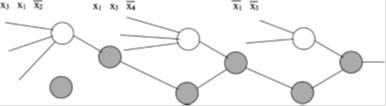
\includegraphics[width=75mm]{arq1.png}
	\caption{Primeira arquitetura proposta}
	\label{arq1}
\end{figure}

Arquitetura 2  - com convergência, e erro próximo a zero em 100\% dos casos (figura \ref{arq2}). 
\begin{figure}[ht!]
	\centering
	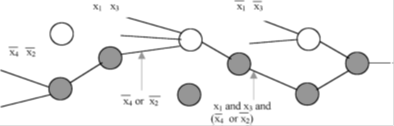
\includegraphics[width=75mm]{arq2.png}
	\caption{Segunda arquitetura proposta}
	\label{arq2}
\end{figure}


Os dados de entrada (x)  e saída (y) forma utilizados conforme o principal arquivo de referência em \cite{pedrycz2006or} e estão organizados na tabela \ref{tab}.

\begin{table}
  \centering
  \begin{tabular}{| l | l | l | l | l | l | l | l | l | l | l | l | l | l | l | l | l |}
  \hline
  x1	& 0	& 0	& 0	& 0	& 0	& 0	& 0	& 1	& 1	& 1	& 1	& 1	& 1	& 1	& 1	& 1 \\
	\hline
  x2	& 0	& 0	& 0	& 0	& 1	& 1	& 1	& 1	& 0	& 0	& 0	& 0	& 1	& 1	& 1	& 1 \\
	\hline
	x3	& 0	& 0	& 1	& 1	& 0	& 0	& 1	& 1	& 0	& 0	& 1	& 1	& 0	& 0	& 1	& 1 \\
	\hline
	x4	& 0	& 1	& 0	& 1	& 0	& 1	& 0	& 1	& 0	& 1	& 0	& 1	& 0	& 1	& 0	& 1 \\
	\hline
	y 	& 1	& 1	& 0	& 0	& 1	& 1	& 0	& 0	& 0	& 0	& 1	& 1	& 0	& 0	& 1	& 0 \\
  \hline
\end{tabular}
  \caption{Dados de entrada}
  \label{tab}
\end{table}

\section{Implementação das funções em MatLab}
Na figura \ref{dig} encontra-se o diagrama de blocos que representa as rotinas construídas para os testes deste trabalho.

\begin{figure}[ht!]
	\centering
	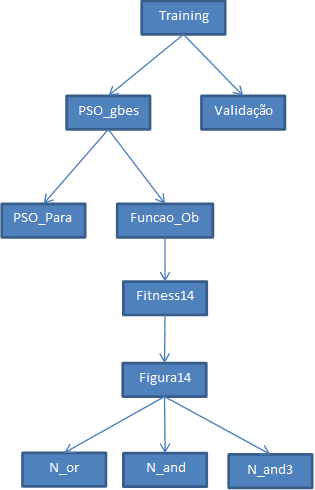
\includegraphics[width=75mm]{dig.png}
	\caption{Diagrama de blocos}
	\label{dig}
\end{figure}

\section{Descrição da Funções:}

\subsection{Training}
Função responsável por efetuar a chamada  ao treinamento da rede e validação dos dados obtidos após o treinamento (pesos).
\subsection{PSO\_gbest}
Função de otimização  responsável por gerar a base de dados aleatória e efetuar a chamada à função objetivo, passando como parâmetro uma matriz com soluções candidatas, esta função será executada até que o critério de parada seja atingido (erro = 0) ou o número de iterações máximo seja atingido.
\subsection{PSO\_parametros}
Parâmetros para execução da função de otimização:
\begin{itemize}
	\item $C = (1,0;0,6)$ - Constantes para pbest e gbest, respecitivamente;
	\item $W = (0,1;0.9]$ - Peso minimo e maximo para as iteracoes;
	\item $n_part = 200$ - Número de particulas;
	\item $iter_max = 500$ - Número maximo de iterações;
	\item $n_var =  9$ - Número de variaveis;
	\item $p_mut = 0.08$ - percentual de operador de diversidade
\end{itemize}
\subsection{Funcao\_Objetivo}
Função responsável por popular $S_k$, ou seja os indivíduos iniciais, para a otimização, onde: 
\begin{itemize}
	\item F:   armazena todos os valores de função objetivo para um determinado
conjunto de valores candidatos a solução.
	\item S\_k:   conjunto de nove pesos por número de soluções candidatas por iteração. 
\end{itemize}
\subsection{Fitness14}
Função responsável por avaliar o conjunto de pesos contidos na matriz S\_k passados a cada iteração da função PSO\_gbest. A função retorna o erro quadrático médio (relacionado a segunda arquitetura proposta da figura 14 do artigo \cite{pedrycz2006or}). 
\subsection{Figura14}
Função que implementa as três camadas propostas no artigo (figura \ref{arq2}) com os parâmetros $x_1$, $x_2$, $x_3$ e $x4$ e os respectivos pesos obtidos na função fitness14. A saída da função é um vetor $Y$, com os valores da tabela \ref{tab}. A função executa a chamada aos neurônios OR e AND implementados nas funções ``n\_or'', ``n\_and'' e``n\_and3'' (também relacionado a segunda arquitetura proposta da figura 14 do artigo \cite{pedrycz2006or}).
\subsection{N\_or}
Função que implementa o neurônio ``OR'' considerando duas entradas ``a,b'' os pesos correspondentes  ``m,n'' e a saída correspondente ``z'', executando o seguinte cálculo da equação \ref{or}: 
\begin{equation} \label{or}
  z = min(max(0, m+a - 1) + max(0, n+b - 1), 1)
\end{equation}
\subsection{N\_and}
Função que implementa o neurônio ``AND'' considerando duas entradas ``a,b'' os pesos correspondentes  ``m,n'' e a saída correspondente ``z'', executando o seguinte cálculo da equação \ref{and}: 
\begin{equation} \label{and}
  z = max(0, min(m+a,1) + min(n+b,1) - 1)
\end{equation}
\subsection{N\_and3}
Função que implementa o neurônio ``AND'' considerando três entradas ``a,b,c'' os pesos correspondentes  ``m,n,p'' e a saída correspondente ``z'' , executando o seguinte cálculo da equação \ref{and3}: 
\begin{equation} \label{and3}
\begin{split}
  z = max(0, max(0, min(m+a,1) + min(n+b,1) - 1)\\
	+ min(p+c,1) - 1
\end{split}
\end{equation}
\subsection{Validação}
	Função que retorna o resultado da rede treinada, ao término do processo de treinamento da  rede, para verificar que a saída corresponde ao conjunto de dados proposto na tabela \ref{tab} do artigo base que é igual à saída do vetor ``y''. 


\section{Conclusão}
Os testes da versão final  da implementação mostraram resultados satisfatórios a partir da iteração de número 60, conforme consta na figura \ref{res}.
\begin{figure}[ht!]
	\centering
	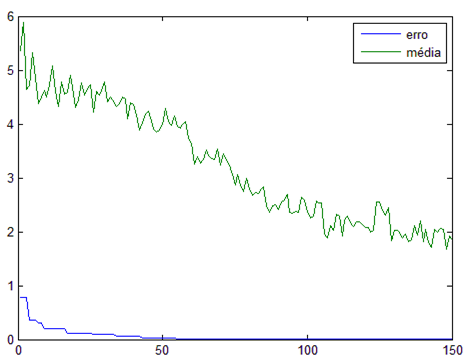
\includegraphics[width=75mm]{res.png}
	\caption{Convergência da rede}
	\label{res}
\end{figure}


% Can use something like this to put references on a page
% by themselves when using endfloat and the captionsoff option.
\ifCLASSOPTIONcaptionsoff
  \newpage
\fi

\bibliographystyle{ieeetran}
\bibliography{bib}

\begin{IEEEbiographynophoto}{Fábio~Juste, Geraldo~Gusmão e Luiz~Le~Roy}
são estudantes do curso de mestrado da Pontif\'icia Universidade Cat\'olica de Minas Gerais.
\end{IEEEbiographynophoto}

% that's all folks
\end{document}
